\newpage
\subsection{Textual; Conditional branching with SDMs}
\texHeader
\hypertarget{conBran tex}{}

Fig.~\ref{fig:cond_branch_on_op_code} depicts the corresponding generated if/else branch in Java.

\begin{figure}[htp]
\begin{center}
  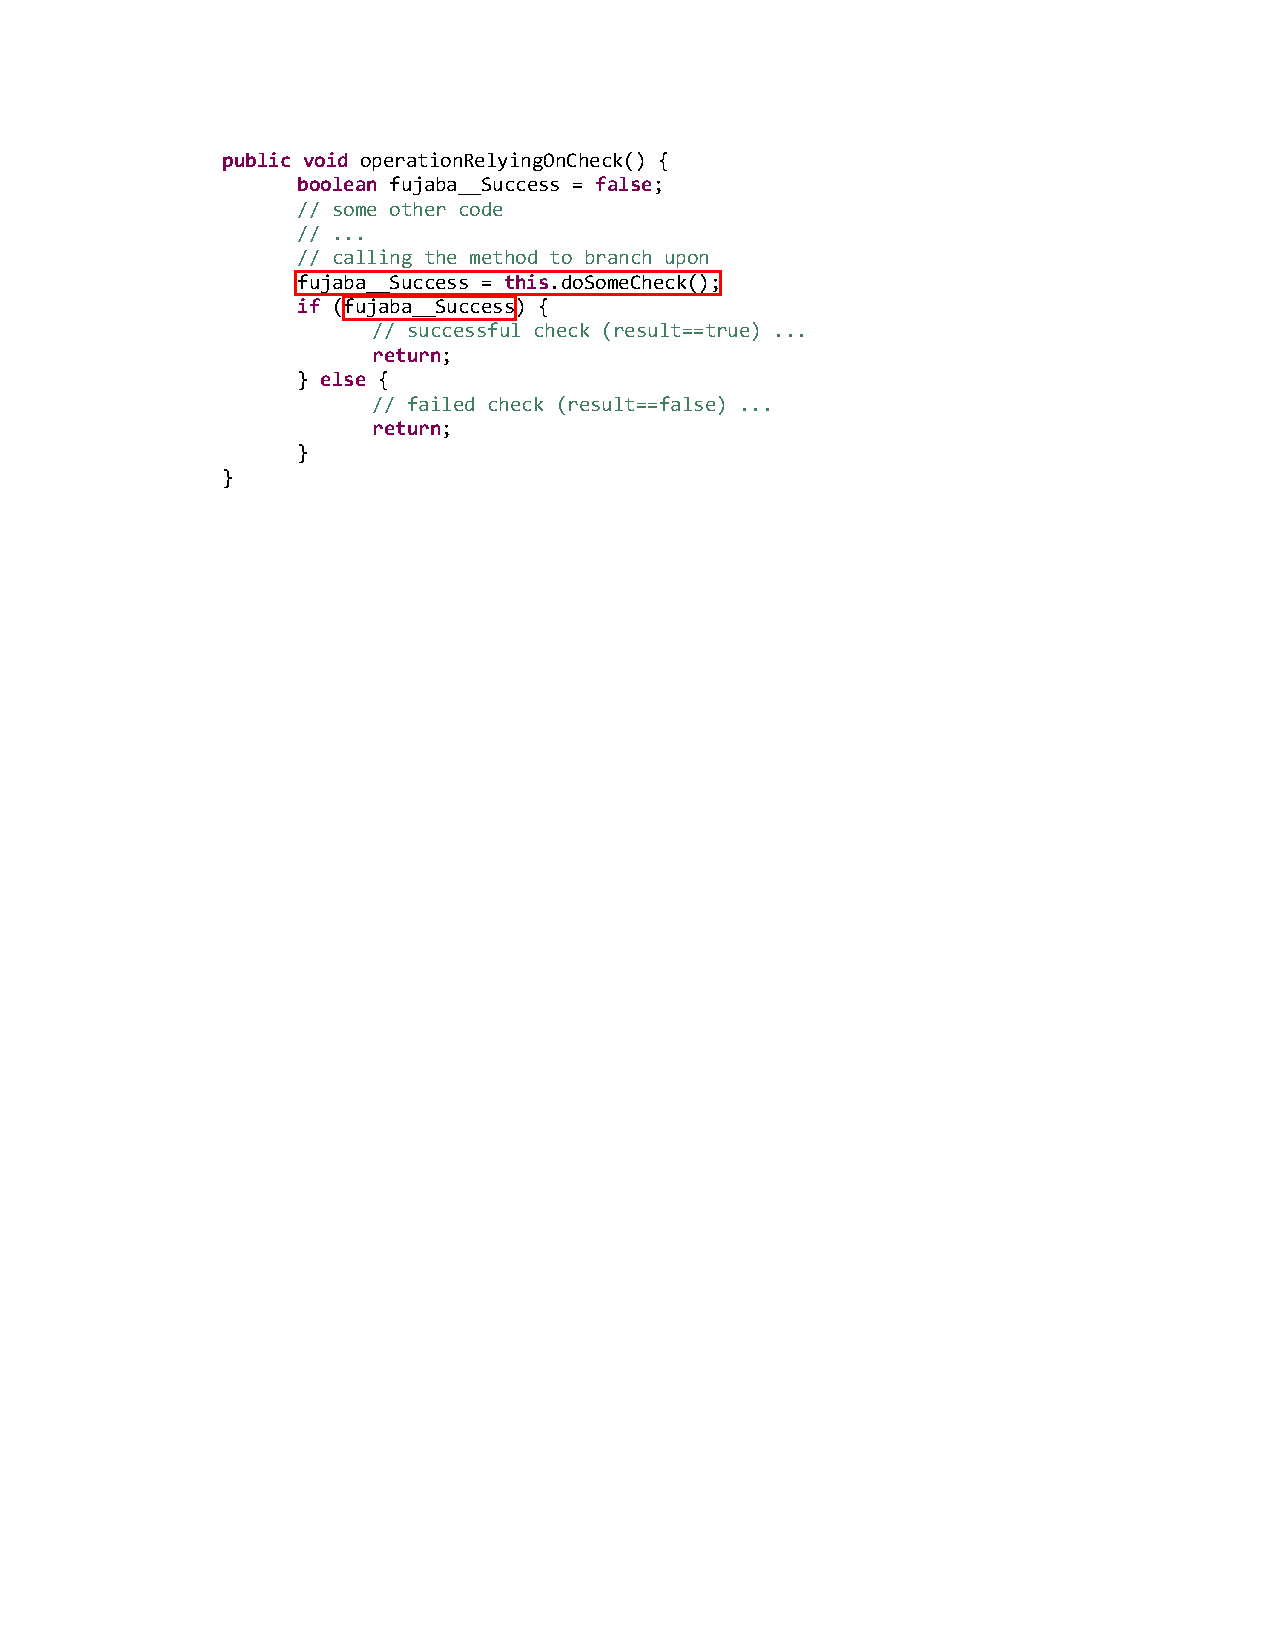
\includegraphics[width=0.7\textwidth]{generated_code}
  \caption{Generated code for branch}
  \label{fig:cond_branch_on_op_code}
\end{center}
\end{figure}

Where should user put this??
